% Chapter 5 — Experimental Results and Analysis
% Every number in this chapter is read from the recorded experiment outputs in
% experiments/final_v2/results; the figures are generated from the same files
% by scripts/make_ch5_figures.py, so figures and tables cannot drift apart.

\section{Introduction}

This chapter reports the experiments that evaluate the trading agents built
in Chapter 4 and interprets their results. The experiments are organised
around five questions that follow directly from the aims of the
dissertation:

\begin{enumerate}
  \item \textbf{Performance.} Do the learned agents outperform appropriate
        non-learning benchmarks on unseen data, net of transaction costs?
  \item \textbf{Behaviour.} Do the learned policies actually condition their
        actions on the observations they are given?
  \item \textbf{State.} Does adding the drawdown feature to the nine-feature
        core state change performance or behaviour?
  \item \textbf{Reward.} Does the risk-aware reward improve the risk--return
        trade-off, rather than merely reducing participation?
  \item \textbf{Robustness.} Do the findings survive different
        transaction-cost assumptions?
\end{enumerate}

The chapter follows the evaluation logic established in Chapter 4: every
design decision is made on the validation months, and the held-out test
months are evaluated once, after all configurations are frozen.
Section~5.2 sets out the protocol, metrics and benchmarks. Section~5.3
calibrates the trade size, a prerequisite for any fair benchmark comparison.
Section~5.4 examines whether the policies use their observations.
Sections~5.5 and~5.6 present the state-representation comparison and the
central held-out results. Sections~5.7 and~5.8 test the risk-aware reward
and transaction-cost sensitivity. Section~5.9 synthesises the findings
against the five questions, and Section~5.10 summarises.

\section{Experimental Protocol and Evaluation Criteria}

This section fixes how every result in the chapter is produced and how the
tables should be read.

\subsection{Data and chronological split}

All experiments use the monthly SPY episodes described in Chapter 4, with
initial capital $C_0 = \$10{,}000$ per episode and a transaction fee of
0.05\% per trade. The 96 months are split chronologically: 2018--2022 for
training (60 months), 2023 for validation (12 months) and 2024--2025 for
testing (24 months). The validation months carry every design decision in
this chapter --- the trade size in Section~5.3 and the risk-penalty weight
in Section~5.7. The test months are evaluated once, in Sections~5.5
to~5.7, after those decisions are frozen.

\subsection{Training and evaluation procedure}

Each configuration trains REINFORCE, Deep Q-learning (DQN) and Proximal
Policy Optimisation (PPO) for 80{,}000 environment steps per seed, with six
random seeds (42--47) per configuration. At evaluation the policies act
deterministically: the policy-gradient methods take their highest-probability
action and the value-based agent its highest-valued action. Before any
trading experiment, the three implementations were verified on standard
reinforcement-learning environments to confirm that the training procedures
operate as expected; those checks are implementation tests rather than
experimental results and are not reported further.

\subsection{Final experimental configurations}

Four learned configurations appear in this chapter, all fixed before the
test pass: the nine-feature core state with the wealth-change reward (the
primary configuration); the ten-feature state adding the drawdown feature,
with the same reward (Question 3); the ten-feature state with the risk-aware
reward (Question 4); and two alternative action models --- whole-share
trades and the uncalibrated $0.10\,C_0$ slice --- retained to confirm the
calibration of Section~5.3 on unseen data.

\subsection{Evaluation metrics}

Five financial quantities are reported per configuration, averaged over
episodes and seeds: the mean wealth change $\Delta W$ in dollars per month;
the mean exposure (the fraction of initial capital held in the asset,
averaged over days); trades per month; the mean intra-episode drawdown; and
the monthly Sharpe ratio. Tables also give the \emph{seed spread}, the gap
between the best and worst of the six seeds. The spread matters as much as
the mean: a spread larger than the mean says the algorithm did not converge
to any single strategy.

One behavioural metric accompanies them. Financial return alone cannot show
whether a policy used its observations, because an unconditional rule can
earn a strong return in a rising market. The \emph{state-dependence
diagnostic} therefore groups every evaluation step by its legal-action mask
pattern. Within one pattern the mask is constant, so if the policy selects
different actions at different steps, the difference can only have come from
the state. A concrete instance: one Deep Q-learning seed met three mask
patterns --- (Hold,\,Buy), (Hold,\,Buy,\,Sell) and (Hold,\,Sell) --- and
chose more than one action inside each of them, so it is
\emph{state-dependent}. A policy that always buys when buying is legal picks
exactly one action per pattern and is labelled \emph{mask-only}: the legal-action
mask, not the market, decides what it does. Tables report how many of the
six seeds were state-dependent.

\subsection{Benchmark strategies}

Four non-learning references are evaluated in the same environment, with the
same accounting and the same fees.

\begin{itemize}
  \item \textbf{Do nothing} holds cash throughout; a lower-bound sanity
        check that anchors $\Delta W = 0$.
  \item \textbf{Buy-and-hold} invests the full capital on day one and
        liquidates at the end of the month. This is the main benchmark. As
        documented in Chapter 4, an earlier implementation accumulated the
        position using the learning agent's transaction size and thereby
        understated the benchmark by \$38.95 per month (21.6\%) on the test
        months; the corrected full-investment version, which beats the
        gradual version in 17 of 24 test months, is used throughout.
  \item \textbf{Always-buy} buys one trade slice every legal day until
        fully invested. It is the strongest strategy available to a policy
        that ignores its observations, which makes it the natural reference
        point when a learned policy collapses to unconditional buying.
  \item \textbf{Random legal} picks uniformly among the currently legal
        actions; a weak stochastic floor.
\end{itemize}

With the protocol fixed, the first experiment asks whether the action model
even permits a fair comparison against the benchmark.

\section{Action-Size Calibration}

The environment executes each Buy or Sell as a fixed transaction amount, so
the size of that amount is an environment parameter, not something the
policy learns. This section shows that the original size made the benchmark
unreachable and calibrates it before any learning comparison.

\subsection{Exposure constraints imposed by the action model}

The trade size decides how fast any agent can build a position. A slice of
$0.10\,C_0$ needs ten buy days to invest fully, but the average episode is
only 20.8 trading days long, so half of a typical month passes before full
investment is even possible. Buy-and-hold faces no such constraint: it is
fully invested from day one. If the action model caps the exposure an agent
can reach, a performance gap against the benchmark may reflect that cap
rather than anything about learning.

\subsection{Validation results for alternative transaction sizes}

To measure the cap directly, a policy that buys at every legal opportunity
was run on the 12 validation months for each candidate slice. No policy at
a given slice can accumulate faster, so its mean exposure is a hard ceiling
for every learned agent using that slice. Table~\ref{tab:slice} and
Figure~\ref{fig:slice} report the ceilings.

\begin{table}[H]
\centering
\caption{Attainable exposure per trade slice on the validation months. The
ceiling policy buys whenever buying is legal; no policy at that slice can
exceed its exposure.}
\label{tab:slice}
\small
\begin{tabular}{@{}lccc@{}}
\toprule
Trade slice & Buy days to full investment & Mean exposure ceiling & Mean $\Delta W$ \\
\midrule
$0.05\,C_0$ & 20 & 0.450 & $+\$95.49$ \\ \rowsep
$0.10\,C_0$ & 10 & 0.690 & $+\$121.79$ \\ \rowsep
$0.25\,C_0$ & 4  & 0.838 & $+\$167.39$ \\ \rowsep
$0.50\,C_0$ & 2  & 0.886 & $+\$162.77$ \\ \rowsep
Buy-and-hold & --- & 0.910 & $+\$166.92$ \\
\bottomrule
\end{tabular}
\end{table}

\begin{figure}[H]
  \centering
  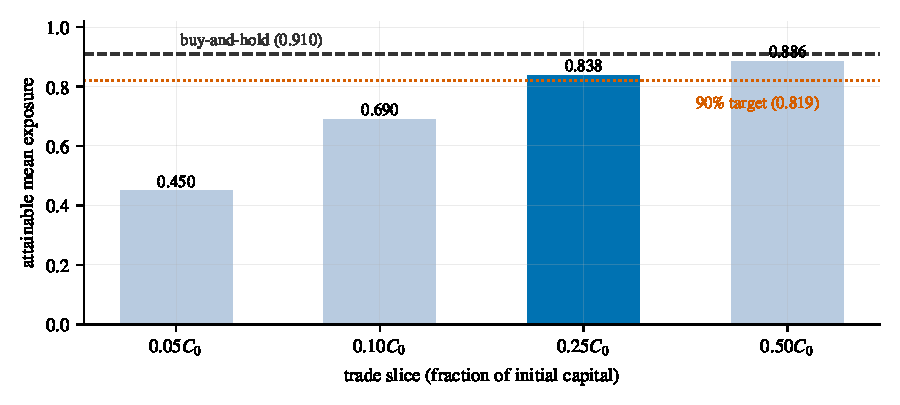
\includegraphics[width=0.82\textwidth]{figs5/fig5_slice.pdf}
  \caption{Exposure ceilings from Table~\ref{tab:slice}. The $0.25\,C_0$
  slice (highlighted) is the smallest that clears the 90\% target of
  buy-and-hold's exposure; the $0.10\,C_0$ slice cannot reach it even in
  principle.}
  \label{fig:slice}
\end{figure}

The $0.10\,C_0$ ceiling is 0.690, only 76\% of buy-and-hold's 0.910. The
consequence is measured in the last column: even a perfect accumulator at
this slice gives up \$45.13 per month against the benchmark ($+\$121.79$
versus $+\$166.92$) before any learning is involved.

\subsection{Selection of the final transaction size}

The selection rule, fixed before looking at the returns, was the smallest
slice whose ceiling reaches 90\% of the benchmark exposure
($0.910 \times 0.9 = 0.819$). The $0.25\,C_0$ slice clears the target with
a ceiling of 0.838; the $0.10\,C_0$ slice does not. The $0.50\,C_0$ slice
climbs slightly higher (0.886) but moves half of all capital per trade,
leaving the agent only two position sizes short of full investment, so it
was not adopted. The primary action model for everything that follows is
therefore $0.25\,C_0$. The original $0.10\,C_0$ slice and a whole-share
variant are retained as test-set comparisons in Section~5.6.5, where the
effect of this choice on unseen data is confirmed.

The action model now gives a learned agent a fair chance. The next question
is behavioural: do the learned policies use the information they observe?

\section{Do the Learned Policies Use Their Observations?}

This section applies the state-dependence diagnostic of Section~5.2.4 to
all three learning methods --- REINFORCE, Deep Q-learning and PPO --- on
the validation months. The experiment runs at both action models: the
calibrated $0.25\,C_0$ slice adopted in Section~5.3, which is the
configuration everything after this point uses, and the original
$0.10\,C_0$ slice, retained so the behavioural conclusion can be checked
against the setting the project started from. If the same pattern appears
at both slices, it is a property of the algorithms rather than an artefact
of the trade size. Every cell was trained from scratch for this study: six
seeds per method per slice, 80{,}000 steps each, on the nine-feature state
and the wealth-change reward exactly as defined in Chapter 3.

\subsection{Behaviour of the learned policies}

Table~\ref{tab:conditioning} summarises all six cells and
Figure~\ref{fig:seeds} shows every seed individually. The columns read as
follows. \emph{Mean $\Delta W$} is the wealth change per month, averaged
first over the 12 validation months and then over the six seeds.
\emph{Seed spread} is the gap between the best and the worst of those six
seeds; a spread larger than the mean says the seeds did not agree on a
strategy. \emph{Exposure} is the fraction of capital invested, averaged
over all days. \emph{Trades} is the mean number of transactions per month.
\emph{State-dependent} counts how many of the six seeds passed the
diagnostic of Section~5.2.4. The always-buy ceiling row in each block is
the always-buy strategy at that trade size: the best any policy that buys
unconditionally can do, and the hard upper bound on exposure.

\begin{table}[H]
\centering
\caption{Conditioning diagnostic on the validation months (nine-feature
state, wealth-change reward, six freshly trained seeds per cell). Each
block reports one action model; its always-buy ceiling row is the maximum
any unconditional buyer at that slice can reach.}
\label{tab:conditioning}
\small
\begin{tabular}{@{}lrrrrc@{}}
\toprule
Policy & Mean $\Delta W$ & Seed spread & Exposure & Trades & State-dependent \\
\midrule
\multicolumn{6}{@{}l}{\emph{Calibrated $0.25\,C_0$ slice}} \\ \rowsep
Always-buy ceiling & $+\$167.39$ & --- & 0.838 & --- & --- \\ \rowsep
REINFORCE & $+\$154.96$ & $\$37.29$ & 0.807 & 10.3 & 0/6 \\ \rowsep
Deep Q-learning & $+\$86.16$ & $\$64.20$ & 0.325 & 8.5 & 6/6 \\ \rowsep
PPO & $+\$118.55$ & $\$167.39$ & 0.596 & 3.7 & 0/6 \\
\midrule
\multicolumn{6}{@{}l}{\emph{Original $0.10\,C_0$ slice}} \\ \rowsep
Always-buy ceiling & $+\$121.79$ & --- & 0.690 & --- & --- \\ \rowsep
REINFORCE & $+\$100.64$ & $\$121.71$ & 0.574 & 15.9 & 0/6 \\ \rowsep
Deep Q-learning & $+\$69.92$ & $\$83.88$ & 0.361 & 12.5 & 6/6 \\ \rowsep
PPO & $+\$112.65$ & $\$54.83$ & 0.631 & 10.0 & 1/6 \\
\bottomrule
\end{tabular}
\end{table}

\begin{figure}[H]
  \centering
  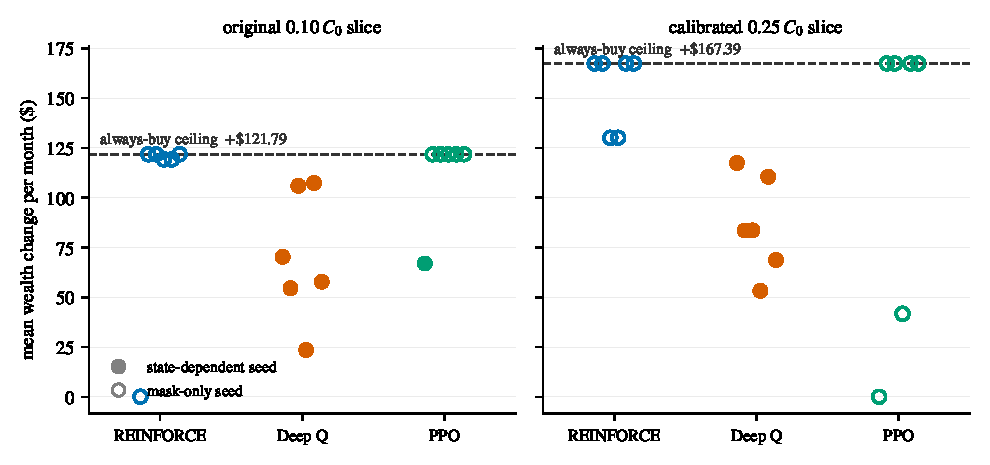
\includegraphics[width=0.95\textwidth]{figs5/fig5_seeds.pdf}
  \caption{Per-seed outcomes behind Table~\ref{tab:conditioning}. Hollow
  markers are mask-only seeds, filled markers state-dependent ones. At
  both slices the policy-gradient methods (REINFORCE, PPO) cluster on the
  always-buy ceiling or collapse towards zero, while all twelve Deep
  Q-learning seeds sit strictly between those corners.}
  \label{fig:seeds}
\end{figure}

At the calibrated slice, the REINFORCE row is best read seed by seed.
Four of its six seeds finished at exactly $+\$167.39$ with exposure 0.838
--- to the cent, the always-buy ceiling of Table~\ref{tab:slice}. They buy
on the first four legal days, hold, and liquidate at month end. The other
two seeds earned $+\$130.10$ while trading 20.8 times per month, once
every bar: a fixed churn pattern that also never consults the market. PPO
split three ways, and its seed spread of \$167.39 measures the full
distance between its corners: four seeds on the ceiling at $+\$167.39$,
one seed that never traded at all ($+\$0.00$, exposure 0.000), and one at
$+\$41.73$ from an unconditional two-trade pattern. Deep Q-learning is the
only method whose seeds avoid both corners: all six sit strictly between,
from $+\$53.23$ to $+\$117.43$, with a mean of $+\$86.16$ at exposure
0.325 --- less than half the attainable 0.838.

The original $0.10\,C_0$ block shows the same shape. REINFORCE put five
seeds on or near that slice's ceiling of $+\$121.79$ and one seed at
$+\$0.08$, so its spread of \$121.71 is again the distance between
always-buy and never-trade, not noise around one strategy. PPO put five
seeds exactly on the ceiling; its remaining seed is the single
state-dependent policy-gradient run in the study ($+\$66.96$). Deep
Q-learning's six seeds again scatter in the interior, from $+\$23.55$ to
$+\$107.43$. Retraining at this slice also reproduced the earlier
exploratory run to the cent for REINFORCE and Deep Q-learning, which
confirms the training pipeline is deterministic given a seed: nothing in
this table is carried over from a previous run.

\subsection{State-dependence analysis}

The final column formalises what the seed plot suggests, and it counts
seeds, not months. A value of 0/6 for REINFORCE means that none of the six
independently retrained REINFORCE policies ever chose different actions in
two situations that had the same legal-action mask. Each of those seeds is
a constant rule: the four ceiling seeds pick Buy whenever Buy is legal,
and the churn seeds alternate on a fixed cycle. The market features could
be replaced by random numbers and these policies would trade identically.
A value of 6/6 for Deep Q-learning means the opposite held for every seed:
each one was observed choosing different actions under an identical mask,
so the difference can only have come from the observed market and
portfolio features. Across the whole study the split is nearly categorical
by algorithm family: twelve of twelve Deep Q-learning seeds were
state-dependent, against one of twenty-four policy-gradient seeds
(REINFORCE and PPO combined, both slices).

\subsection{Interpretation of the learned trading behaviour}

The split in Table~\ref{tab:conditioning} follows from how each algorithm
learns. REINFORCE and PPO adjust action probabilities directly in the
direction of sampled returns. On training years where buying generally
paid, every update raises the probability of Buy in all states at once,
because the return signal says which action was good, not which
observation justified it. Once the policy is nearly deterministic,
exploration disappears with it: a policy that buys with probability close
to one almost never samples the alternatives that could correct it. The
corner outcomes are exactly what this predicts. Seeds of both
policy-gradient methods finish on the always-buy ceiling to the cent, and
the PPO seed that never traded shows the same collapse with the opposite
sign: early negative samples pushed its trading probability towards zero,
and exploration died before the estimate could recover.

Deep Q-learning is built differently. It learns a separate value estimate
for each action as a function of the observed state, and its policy picks
the action with the highest estimate at each step. Whenever those
estimates cross as the features change, the chosen action changes with
them, so state-dependent behaviour is a structural property of the method
rather than an achievement. Its $\epsilon$-greedy exploration is also
imposed from outside the policy, so it keeps sampling alternative actions
no matter how settled the value estimates become. The diagnostic cannot
certify that these responses are useful, however: the calibrated-slice
seeds scatter from $+\$53.23$ to $+\$117.43$, which says each seed
learned different entry and exit thresholds and none of them timed the
2023 market well.

These mechanisms are interpretations: the experiments show the behaviour,
not its internal cause. They are, however, consistent with every detail
of Table~\ref{tab:conditioning}, at both trade sizes --- exact ceiling
replication by the policy-gradient seeds, collapse in both directions,
and interior scatter for the value-based method. The market then set the
payoffs. The validation year of 2023 generally rose, so the mask-only
strategies that stayed invested earned within \$12.43 of the calibrated
ceiling, while the one method that stepped in and out of the market
earned \$81.23 per month less. Using the state was not rewarded on these
months, and the same asymmetry recurs on the held-out test months in
Section~5.6. The next section turns to the state itself: does the
drawdown feature change any of this?

\section{Effect of the State Representation}

Chapter 3 justified the nine-feature core state by design argument and
reserved the tenth feature, the running drawdown, for the risk-aware
experiments. This section isolates the state axis empirically: same
wealth-change reward, same $0.25\,C_0$ action model, only the state
differs. Both configurations were frozen before the single test pass, and
the comparison uses the 24 held-out months. The question is deliberately
narrow: does adding drawdown information alone change the learned policy?

\begin{table}[H]
\centering
\caption{Effect of the state representation on the held-out test months
(wealth-change reward, $0.25\,C_0$ slice, six seeds). DD is mean
intra-episode drawdown; State-dep.\ counts state-dependent seeds.}
\label{tab:state}
\small
\begin{tabular}{@{}llrrrrrrc@{}}
\toprule
Method & State & $\Delta W$ (\$) & Spread & Exposure & Trades & DD & Sharpe & State-dep. \\
\midrule
REINFORCE & 9-feature  & $+171.51$ & 24.7  & 0.810 & 10.3 & 0.0266 & 0.675 & 0/6 \\ \rowsep
REINFORCE & 10-feature & $+167.39$ & 24.7  & 0.794 & 13.0 & 0.0263 & 0.670 & 0/6 \\ \rowsep
Deep Q    & 9-feature  & $+74.68$  & 71.4  & 0.312 & 8.2  & 0.0124 & 0.507 & 6/6 \\ \rowsep
Deep Q    & 10-feature & $+77.81$  & 89.5  & 0.354 & 7.4  & 0.0140 & 0.505 & 6/6 \\ \rowsep
PPO       & 9-feature  & $+127.35$ & 179.8 & 0.598 & 3.7  & 0.0195 & 0.562 & 0/6 \\ \rowsep
PPO       & 10-feature & $+159.97$ & 94.0  & 0.759 & 7.3  & 0.0250 & 0.671 & 1/6 \\
\bottomrule
\end{tabular}
\end{table}

\begin{figure}[H]
  \centering
  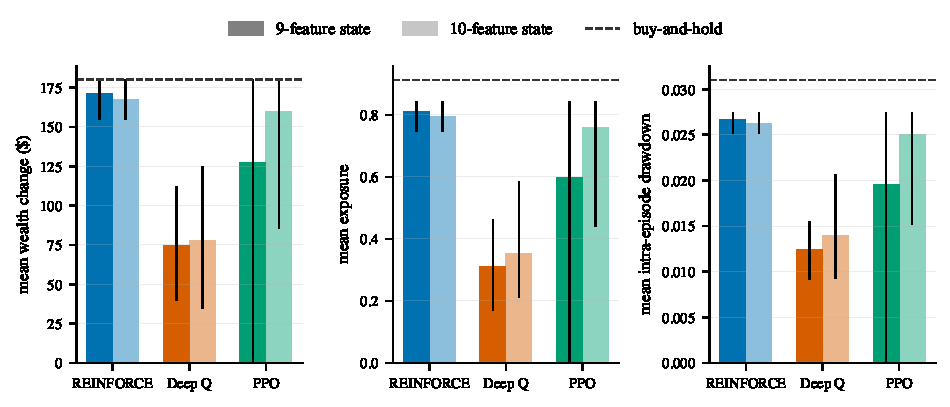
\includegraphics[width=0.78\textwidth]{figs5/fig5_state.pdf}
  \caption{Return, exposure and drawdown under the two states; whiskers
  span the best and worst seed and the dashed line marks buy-and-hold.
  Every 9-to-10-feature difference is smaller than the corresponding
  whisker range, and all three quantities move together.}
  \label{fig:state}
\end{figure}

\subsection{Comparison of the core and risk-aware states}

For the two methods with interpretable behaviour, the tenth feature moved
the outcome by less than the seed noise. REINFORCE changed by $-\$4.12$
per month ($+\$171.51$ to $+\$167.39$) against a seed spread of \$24.70;
Deep Q-learning changed by $+\$3.13$ ($+\$74.68$ to $+\$77.81$) against
spreads of \$71.40 and \$89.50. Both shifts are roughly one-sixth of the
corresponding spread or less, so neither is distinguishable from the
variation between seeds. The state-dependence column is equally stable:
REINFORCE remained mask-only (0/6) and Deep Q-learning fully
state-dependent (6/6) under both states.

PPO appears to improve, from $+\$127.35$ to $+\$159.97$, a gain of
\$32.62. That number needs its spread read alongside it: \$179.80 under the
nine-feature state --- larger than the mean itself --- narrowing to \$94.00
under ten features, with just one seed in six becoming state-dependent. A
difference of \$32.62 between two configurations whose individual seeds
range over \$94--\$180 cannot be attributed to the extra feature; it is
within the movement that reseeding alone produces.

\subsection{Analysis of return, exposure and risk}

The supporting columns tell the same story in different units. Deep
Q-learning's exposure rose from 0.312 to 0.354 and its drawdown from 0.0124
to 0.0140 when the feature was added --- return, exposure and risk all
moved up together by similar proportions, which is the signature of
slightly larger positions, not of different decisions. Its Sharpe ratio is
flat (0.507 against 0.505). REINFORCE's columns barely move at all, as
expected for a policy family that does not read the state it is given.

\subsection{Interpretation of the state-representation results}

The experiments did not demonstrate a consistent performance improvement
from adding drawdown information to the core state. This does not imply
that the nine-feature state is universally sufficient, nor that the
drawdown feature is badly designed. It means that, within this environment
and under the wealth-change objective, the additional information did not
provide a measurable advantage --- an agent maximising wealth change in
generally rising markets has little use for its own loss history. The
feature becomes decision-relevant only when the objective makes drawdown
costly, which is precisely the pairing tested in Section~5.7. Before that,
the next section presents the central comparison this chapter exists to
report.

\section{Held-Out Test Results}

This section answers the first research question: how does each learned
strategy, in its final configuration, compare with the non-learning
benchmarks on unseen data? The configuration is the one frozen on
validation --- nine-feature state, wealth-change reward, $0.25\,C_0$ slice
--- evaluated once over the 24 test months of 2024--2025.
Table~\ref{tab:test} is the central result of the dissertation.

\begin{table}[H]
\centering
\caption{Held-out test results over 24 months (2024--2025): benchmarks and
the three learned agents in the final configuration, six seeds each.}
\label{tab:test}
\small
\begin{tabular}{@{}lrrrrrrc@{}}
\toprule
Policy & $\Delta W$ (\$) & Spread & Exposure & Trades & DD & Sharpe & State-dep. \\
\midrule
Do nothing     & $0.00$    & --- & 0.000 & 0.0  & 0.0000 & ---   & --- \\ \rowsep
Buy-and-hold   & $+180.25$ & --- & 0.913 & 2.0  & 0.0310 & 0.638 & --- \\ \rowsep
Always-buy ($0.25\,C_0$) & $+179.75$ & --- & 0.841 & 5.0  & 0.0274 & 0.684 & --- \\ \rowsep
Random legal   & $+22.73$  & --- & 0.304 & 13.3 & 0.0133 & 0.124 & --- \\ \rowsep
REINFORCE      & $+171.51$ & 24.7  & 0.810 & 10.3 & 0.0266 & 0.675 & 0/6 \\ \rowsep
Deep Q-learning& $+74.68$  & 71.4  & 0.312 & 8.2  & 0.0124 & 0.507 & 6/6 \\ \rowsep
PPO            & $+127.35$ & 179.8 & 0.598 & 3.7  & 0.0195 & 0.562 & 0/6 \\
\bottomrule
\end{tabular}
\end{table}

\subsection{Overall comparison with the benchmark strategies}

Buy-and-hold earned $+\$180.25$ per month, and no learned agent exceeded
it. The closest was REINFORCE at $+\$171.51$, a shortfall of \$8.74 per
month; Deep Q-learning earned $+\$74.68$ and PPO $+\$127.35$. Over the
full two years the gap compounds visibly in Figure~\ref{fig:cumwealth}:
buy-and-hold accumulates $+\$4{,}326$ of monthly wealth changes, REINFORCE
$+\$4{,}116$, PPO $+\$3{,}056$ and Deep Q-learning $+\$1{,}792$. All three
learned agents clear the random-legal floor ($+\$22.73$ per month) by a
wide margin, so the learning is doing something; the question the following
subsections answer is what.

\begin{figure}[H]
  \centering
  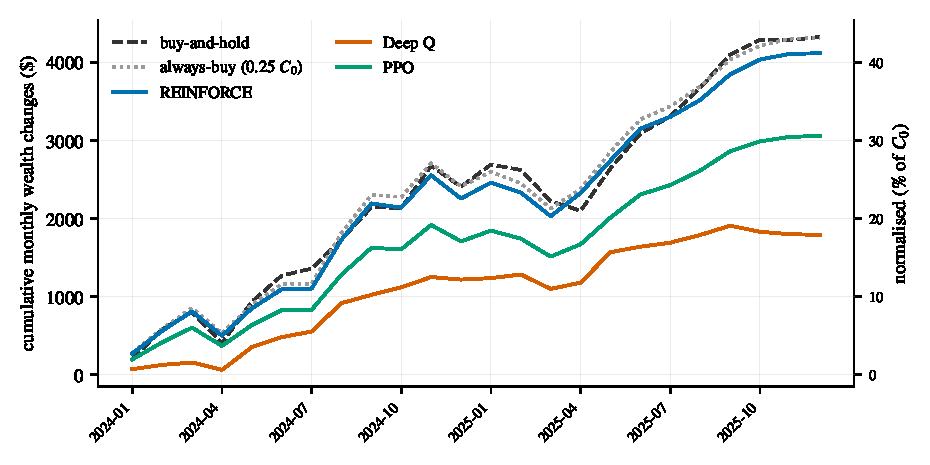
\includegraphics[width=0.92\textwidth]{figs5/fig5_cumwealth.pdf}
  \caption{Cumulative sum of mean monthly wealth changes over the test
  months (episodes reset to $C_0$ each month, so the curves accumulate
  monthly results rather than compound; the right axis reads the same
  values as a percentage of $C_0$). REINFORCE tracks the always-buy reference
  and buy-and-hold almost exactly; Deep Q-learning's low exposure keeps
  its curve flattest, including through the March--April 2025 drawdown.}
  \label{fig:cumwealth}
\end{figure}

\subsection{Return and market exposure}

The exposure column explains most of the return column. REINFORCE held
exposure 0.810 and its whole row --- return, drawdown 0.0266, Sharpe 0.675,
and 0 of 6 state-dependent seeds --- sits within a few percent of
Always-buy ($0.25\,C_0$): $+\$179.75$, 0.841, 0.0274, 0.684, the
unconditional strategy that buys every legal day. Its tight spread of \$24.70, the smallest of any
learned cell, is the spread of a policy family that has stopped depending
on anything the market does. The $+\$171.51$ is therefore the return of
committed participation in two rising years, not evidence of market
timing. Deep Q-learning, the one method whose seeds all condition on the
state, chose to participate least: exposure 0.312, roughly a third of the
benchmark's 0.913, and its return is correspondingly roughly a third.

\subsection{Risk and risk-adjusted performance}

Whether an agent that earns less has at least found a better way to take
risk is a question about efficiency, and Figure~\ref{fig:effic} puts every
learned configuration in the chapter on that scale. Buy-and-hold earned
\$197 per unit of exposure. An agent that merely holds less of the same
asset lands on the dashed proportional line; genuine downside management
would appear above it.

\begin{figure}[H]
  \centering
  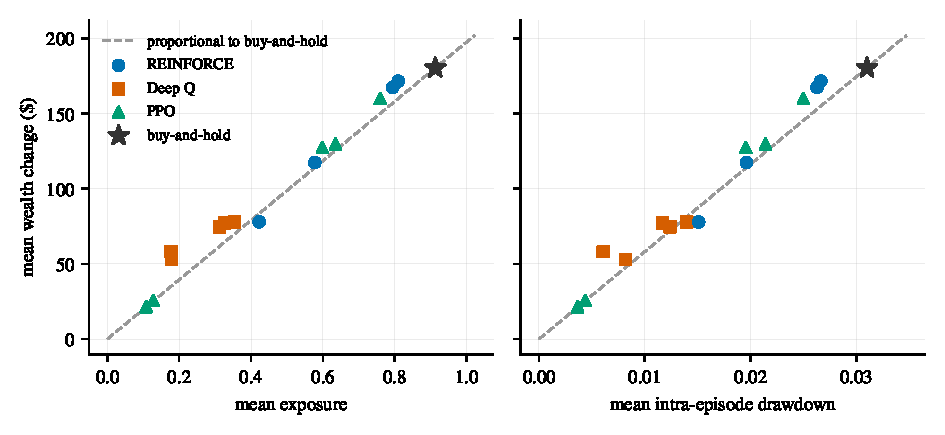
\includegraphics[width=0.95\textwidth]{figs5/fig5_effic.pdf}
  \caption{Mean wealth change against exposure (left) and against
  intra-episode drawdown (right) for every learned configuration in this
  chapter. The dashed lines are proportional scalings of buy-and-hold. No
  learned configuration sits meaningfully above either line.}
  \label{fig:effic}
\end{figure}

Deep Q-learning is the informative case, because it is the only agent whose
behaviour could in principle express timing skill. It earned 41.4\% of the
benchmark's return at 34.2\% of its exposure and 40.0\% of its drawdown ---
return and risk fell by the same factor as participation, which is what
scaling down does. Its Sharpe ratio of 0.507 against buy-and-hold's 0.638
confirms it earned \emph{less} return per unit of risk, not more.

A single month makes the mechanism concrete. March 2025 was the worst test
month for the benchmark: buy-and-hold lost \$398.41 with an intra-month
drawdown of 5.6\%. If the state-dependent agent had recognised the
conditions, that is the month to step aside. Instead Deep Q-learning held
a mean exposure of 0.490 that month --- \emph{above} its overall average of
0.312 --- and lost \$184.04, which is 46\% of the benchmark's loss. Even
in the month where avoidance was most valuable, the loss matched the
participation. The lower drawdown in
Table~\ref{tab:test} is bought by holding less, not by knowing when.

Figure~\ref{fig:months} extends that single month to all 24. Each pair of
bars is one test month: the dark bar is buy-and-hold's wealth change and
the orange bar is the Deep Q-learning seed mean for the same month. The
two series rise and fall together --- the agent's best month is the
benchmark's best month (May 2025, $+\$390.80$ against $+\$543.11$) and its
worst is the benchmark's worst (the highlighted March 2025). Buy-and-hold
lost money in seven of the 24 months, and the agent ended positive in
three of those seven. Those three, however, were the mildest, with
benchmark losses of only \$9.64, \$69.99 and \$124.50 --- small enough for
intra-month trading to finish ahead without any foresight. In the two
heavy down months, April 2024 ($-\$396.08$) and March 2025 ($-\$398.41$),
the agent captured 24\% and 46\% of the benchmark's loss, bracketing its
34\% average participation. Where downside management mattered most, the
losses again tracked the exposure.

\begin{figure}[H]
  \centering
  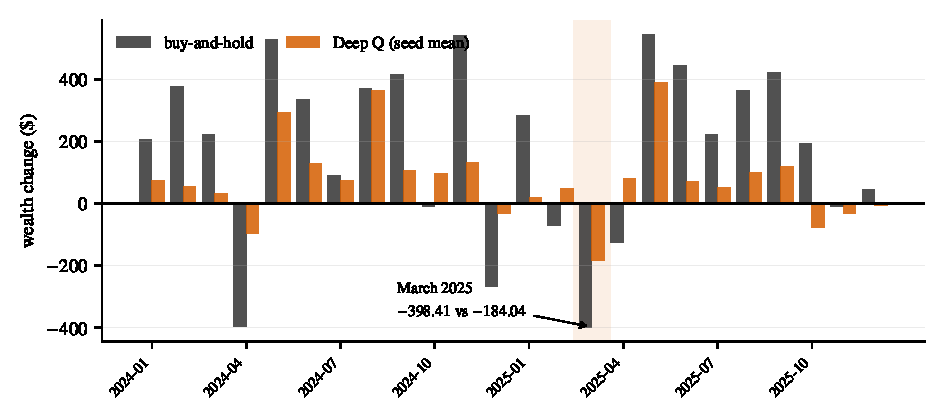
\includegraphics[width=0.95\textwidth]{figs5/fig5_months.pdf}
  \caption{Monthly wealth changes of buy-and-hold and Deep Q-learning
  (seed mean) over the 24 test months. The agent's bars are a scaled copy
  of the benchmark's in almost every month; in the highlighted March 2025,
  the worst month, it lost \$184.04 against the benchmark's \$398.41.}
  \label{fig:months}
\end{figure}

Figure~\ref{fig:mscatter} compresses the same comparison into one plot.
Each point is one test month, placing the agent's wealth change (vertical)
against the benchmark's (horizontal); the dashed line is what pure
scaled-down participation at the agent's exposure ratio of 0.34 would
produce. A line through the origin fitted to the 24 points has slope 0.36
and explains 63\% of the month-to-month variance, so the agent's monthly
result is, on average, one-third of the benchmark's result in whichever
direction the market moved. Downside timing skill would bend the pattern:
points in the left half of the plot (benchmark losing) would sit well
above the dashed line while points in the right half stayed on it. No
such bend is visible. The points that do sit above the line on the left
are the three mild down months already identified, and the two large-loss
months sit on or below it.

\begin{figure}[H]
  \centering
  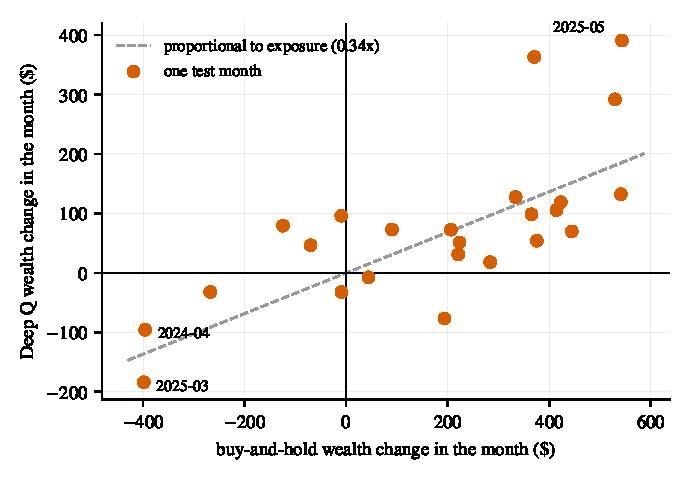
\includegraphics[width=0.62\textwidth]{figs5/fig5_mscatter.pdf}
  \caption{Deep Q-learning's monthly wealth change against buy-and-hold's
  for the same month, one point per test month. The dashed line is
  proportional participation at the agent's exposure ratio (0.34). The
  fitted through-origin slope is 0.36 ($R^2 = 0.63$): monthly results
  scale with exposure in both directions, with no asymmetry in the
  large-loss months where timing skill would show.}
  \label{fig:mscatter}
\end{figure}

\subsection{Trading behaviour and consistency across seeds}

The spread column qualifies every mean above. PPO's spread of \$179.80
exceeds its own mean of $+\$127.35$: individual seeds ranged from
near-inactivity to near-full investment, and none conditioned on the state.
REINFORCE's seeds agree with each other (spread \$24.70) precisely because
they agree on ignoring the market. Deep Q-learning sits between
(\$71.40). Two practical conclusions follow: single-seed results in this
domain border on anecdote, and a small spread is not by itself evidence of
good behaviour --- REINFORCE's spread is small because its policy is
degenerate.

\subsection{Sensitivity to the action model}

The last comparison confirms the calibration of Section~5.3 on unseen
data. Table~\ref{tab:action} re-runs the same learned configuration under
the uncalibrated $0.10\,C_0$ slice and a whole-share action model, each
with its own accumulation reference.

\begin{table}[H]
\centering
\caption{Effect of the action model on the held-out months (nine-feature
state, wealth-change reward). Each block lists the always-buy reference
for that action model, then the learned agents.}
\label{tab:action}
\small
\begin{tabular}{@{}llrrrrrr@{}}
\toprule
Action model & Policy & $\Delta W$ (\$) & Spread & Exposure & Trades & DD & Sharpe \\
\midrule
$0.25\,C_0$ (calibrated) & Always-buy & $+179.75$ & ---   & 0.841 & 5.0  & 0.0274 & 0.684 \\ \rowsep
$0.25\,C_0$ (calibrated) & REINFORCE      & $+171.51$ & 24.7  & 0.810 & 10.3 & 0.0266 & 0.675 \\ \rowsep
$0.25\,C_0$ (calibrated) & Deep Q         & $+74.68$  & 71.4  & 0.312 & 8.2  & 0.0124 & 0.507 \\ \rowsep
$0.25\,C_0$ (calibrated) & PPO            & $+127.35$ & 179.8 & 0.598 & 3.7  & 0.0195 & 0.562 \\ \rowsep
$0.10\,C_0$ & Always-buy & $+141.31$ & ---   & 0.694 & 11.0 & 0.0235 & 0.616 \\ \rowsep
$0.10\,C_0$ & REINFORCE      & $+117.40$ & 132.4 & 0.578 & 15.9 & 0.0196 & 0.550 \\ \rowsep
$0.10\,C_0$ & Deep Q         & $+77.37$  & 42.9  & 0.327 & 11.2 & 0.0117 & 0.504 \\ \rowsep
$0.10\,C_0$ & PPO            & $+129.74$ & 69.4  & 0.635 & 10.0 & 0.0214 & 0.627 \\ \rowsep
Whole share & Always-buy & $+94.69$  & ---   & 0.502 & 18.1 & 0.0178 & 0.559 \\ \rowsep
Whole share & REINFORCE      & $+77.91$  & 99.8  & 0.422 & 19.0 & 0.0151 & 0.427 \\ \rowsep
Whole share & Deep Q         & $+58.23$  & 61.6  & 0.177 & 10.4 & 0.0061 & 0.541 \\ \rowsep
Whole share & PPO            & $+25.75$  & 90.1  & 0.128 & 4.8  & 0.0044 & 0.211 \\
\bottomrule
\end{tabular}
\end{table}

The action model moved returns far more than the state representation did.
The whole-share model cut REINFORCE from $+\$171.51$ to $+\$77.91$
($-\$93.60$) and PPO from $+\$127.35$ to $+\$25.75$ ($-\$101.60$); even the
unconditional accumulation reference fell to $+\$94.69$, because one share
per day cannot build a meaningful position within a month. Reverting to
the $0.10\,C_0$ slice cut REINFORCE by \$54.11 and multiplied its spread
by five (from \$24.70 to \$132.40). Every one of these swings exceeds the
largest state-representation effect in Table~\ref{tab:state}
(\$32.62) by a factor of two to three, which confirms that the action
model is part of the problem definition, not an implementation detail.
Had the dissertation compared learned agents to buy-and-hold at the
original $0.10\,C_0$ slice, the resulting gap would have measured the
action constraint, not the learning.

The central comparison leaves one designed capability untested: the
risk-aware reward. The next section evaluates it.

\section{Effect of the Risk-Aware Reward}

This section answers the fourth research question. Chapter~3 defined the
risk-aware reward as
\[
r^{\mathrm{risk}}_t \;=\; \Delta W_t \;-\; \lambda\, C_0\, \Delta dd_t,
\]
where \(\Delta dd_t\) is the increase in running drawdown at step \(t\)
(and is zero when drawdown does not rise), and the \(C_0\) factor puts
both terms in dollars so that \(\lambda\) is dimensionless. With
\(\lambda = 0\) this is exactly the wealth-change reward. The reward is
paired with the ten-feature state throughout, since the penalised
quantity must be observable for the process to remain a Markov decision
process.

\subsection{Selection of the penalty weight}

The weight was selected on the validation months only, using Deep
Q-learning as the selector because it is the only method whose policies
consistently respond to the state (Section~5.4).

The rule declared before the sweep --- accept the largest $\lambda$ whose
validation mean stays within one seed spread of the unpenalised agent ---
failed in an instructive way. The unpenalised mean was $+\$78.35$ but the
seed spread was \$106.94, so the acceptance floor worked out to
$-\$28.59$: a \emph{negative} return would have passed. Every value in the
grid cleared that floor, the rule selected $\lambda = 2.0$, and the
resulting agents simply stopped trading; on the test months, all three
methods at $\lambda = 2.0$ recorded $\Delta W \approx \$0.00$ with zero
trades. When the seed spread exceeds the mean, a spread-based tolerance
tolerates total inactivity.

The revised rule requires the penalised agent to retain at least half of
the unpenalised mean return (at least $+\$39.17$) and half of the
unpenalised exposure (at least 0.223). Table~\ref{tab:lambda} and
Figure~\ref{fig:lambda} show the sweep against those floors.

\begin{table}[H]
\centering
\caption{Risk-penalty sweep on the validation months (Deep Q-learning, six
seeds). The revised rule requires $\Delta W \ge +\$39.17$ and exposure
$\ge 0.223$; the largest passing value is $\lambda = 0.10$.}
\label{tab:lambda}
\small
\begin{tabular}{@{}rrrrrc@{}}
\toprule
$\lambda$ & Mean $\Delta W$ & Exposure & Drawdown & DD change & Passes \\
\midrule
0 (unpenalised) & $+\$78.35$ & 0.445 & 0.0163 & ---        & --- \\ \rowsep
0.05 & $+\$88.78$ & 0.401 & 0.0128 & $-21.5\%$  & yes \\ \rowsep
0.10 & $+\$67.30$ & 0.344 & 0.0124 & $-24.0\%$  & yes \\ \rowsep
0.25 & $+\$19.90$ & 0.074 & 0.0035 & $-78.4\%$  & no  \\ \rowsep
0.50 & $+\$1.73$  & 0.002 & 0.0001 & $-99.4\%$  & no  \\ \rowsep
1.00 & $\$0.00$   & 0.000 & 0.0000 & $-100\%$   & no  \\ \rowsep
2.00 & $\$0.00$   & 0.000 & 0.0000 & $-100\%$   & no  \\
\bottomrule
\end{tabular}
\end{table}

\begin{figure}[H]
  \centering
  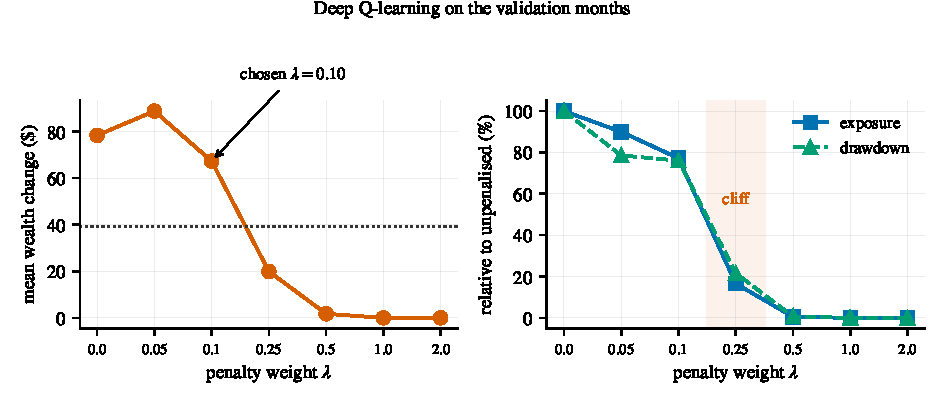
\includegraphics[width=0.8\textwidth]{figs5/fig5_lambda.pdf}
  \caption{The sweep of Table~\ref{tab:lambda}. Left: mean wealth change
  against $\lambda$ with the selection floor of $+\$39.17$. Right:
  exposure and drawdown as percentages of their unpenalised values ---
  between $\lambda = 0.10$ and $0.25$ participation collapses rather than
  declines.}
  \label{fig:lambda}
\end{figure}

The sweep is a cliff, not a slope. Between $\lambda = 0.10$ and $0.25$,
exposure collapses from 0.344 to 0.074 --- a 78\% drop for a 2.5$\times$
increase in the penalty --- and by $\lambda = 0.50$ the agent holds
essentially nothing (exposure 0.002). The mechanism is plain: a policy
that never holds the asset can never draw down, so once the penalty
outweighs the upside of participating, the cheapest optimum is abstinence.
The largest value satisfying both floors is $\lambda = 0.10$, which was
frozen and carried to the test set.

\subsection{Effect on the held-out test set}

Table~\ref{tab:risk} isolates the reward axis: same ten-feature state, same
action model, only the reward differs.

\begin{table}[H]
\centering
\caption{Wealth-change versus risk-aware reward ($\lambda = 0.10$) on the
held-out months, ten-feature state, six seeds.}
\label{tab:risk}
\small
\begin{tabular}{@{}llrrrrrr@{}}
\toprule
Method & Reward & $\Delta W$ (\$) & Spread & Exposure & Trades & DD & Sharpe \\
\midrule
REINFORCE & wealth & $+167.39$ & 24.7  & 0.794 & 13.0 & 0.0263 & 0.670 \\ \rowsep
REINFORCE & risk   & $+167.39$ & 24.7  & 0.794 & 13.0 & 0.0263 & 0.670 \\ \rowsep
Deep Q    & wealth & $+77.81$  & 89.5  & 0.354 & 7.4  & 0.0140 & 0.505 \\ \rowsep
Deep Q    & risk   & $+52.90$  & 43.1  & 0.178 & 5.4  & 0.0082 & 0.416 \\ \rowsep
PPO       & wealth & $+159.97$ & 94.0  & 0.759 & 7.3  & 0.0250 & 0.671 \\ \rowsep
PPO       & risk   & $+21.48$  & 128.9 & 0.108 & 0.7  & 0.0037 & 0.107 \\
\bottomrule
\end{tabular}
\end{table}

For Deep Q-learning the penalty cut drawdown from 0.0140 to 0.0082, a 41\%
reduction. But return fell from $+\$77.81$ to $+\$52.90$ (32\%) and
exposure from 0.354 to 0.178 (50\%), so the risk saving was bought with
participation, and the Sharpe ratio dropped from 0.505 to 0.416. PPO
reacted more severely: exposure 0.108, fewer than one trade per month, and
a return of $+\$21.48$ --- barely ahead of the random-legal reference.
REINFORCE did not react at all: its two rows are identical, which is
exactly what one expects when a policy has collapsed to an unconditional
rule --- changing the reward changes the gradient signal, but the converged
behaviour never consulted the penalised quantity in the first place.

\subsection{The return--risk trade-off}

The decisive question is not whether drawdown decreased --- a sufficiently
large penalty guarantees that, trivially, by ending participation. The
question is whether any agent retained a meaningful level of return and
exposure while reducing risk, and the answer in Table~\ref{tab:risk} is
no: every reduction in drawdown was accompanied by an equal or larger
reduction in exposure and return, and Sharpe ratios fell in every case
where behaviour changed. In Figure~\ref{fig:effic}, the risk-reward
configurations are the points nearest the origin --- further down the
proportional line, not above it. This is a limitation of the penalty's
form rather than of risk-aware learning as an idea: a subtraction
proportional to drawdown gives the agent one easy lever, participation,
and it pulls it. Objectives that reward return earned per unit of risk are
identified as future work in Chapter 6.

\section{Transaction-Fee Sensitivity}

The 0.05\% fee used everywhere else is an assumption, and a result that
only survives at an optimistic cost level is not a result. This section
varies the fee from 0 to 50 basis points
(0bps($0.00\%$) to 50bps($0.50\%$)) on the validation months with the
nine-feature state, everything else held fixed. The sweep was run for all
three learners --- REINFORCE, Deep Q-learning and PPO --- each with six
freshly trained seeds per fee level.
Table~\ref{tab:fees} and Figure~\ref{fig:fees} report the outcome.

\begin{table}[H]
\centering
\caption{Fee sensitivity on the validation months (six seeds per learned
cell). Trades are per month. Fees are shown in basis points and as a
percentage of trade value; 5bps($0.05\%$) is the default used elsewhere.}
\label{tab:fees}
\small
\begin{tabular}{@{}lrrrrrrr@{}}
\toprule
Fee & B\&H $\Delta W$ & REINF.\ $\Delta W$ & REINF.\ trades &
Deep Q $\Delta W$ & Deep Q trades & PPO $\Delta W$ & PPO trades \\
\midrule
0bps($0.00\%$)  & $+\$177.09$ & $+\$177.56$ & 5.0  & $+\$108.00$ & 10.9 & $+\$155.35$ & 4.5 \\ \rowsep
5bps($0.05\%$)  & $+\$166.92$ & $+\$154.96$ & 10.3 & $+\$86.16$  & 8.5  & $+\$118.55$ & 3.7 \\ \rowsep
10bps($0.10\%$) & $+\$156.76$ & $+\$143.74$ & 4.7  & $+\$77.60$  & 8.9  & $+\$78.50$  & 2.7 \\ \rowsep
25bps($0.25\%$) & $+\$126.33$ & $+\$88.76$  & 10.3 & $+\$32.35$  & 3.9  & $+\$26.40$  & 1.2 \\ \rowsep
50bps($0.50\%$) & $+\$75.83$  & $+\$41.31$  & 2.8  & $+\$16.32$  & 1.9  & $+\$12.60$  & 1.0 \\
\bottomrule
\end{tabular}
\end{table}

\begin{figure}[H]
  \centering
  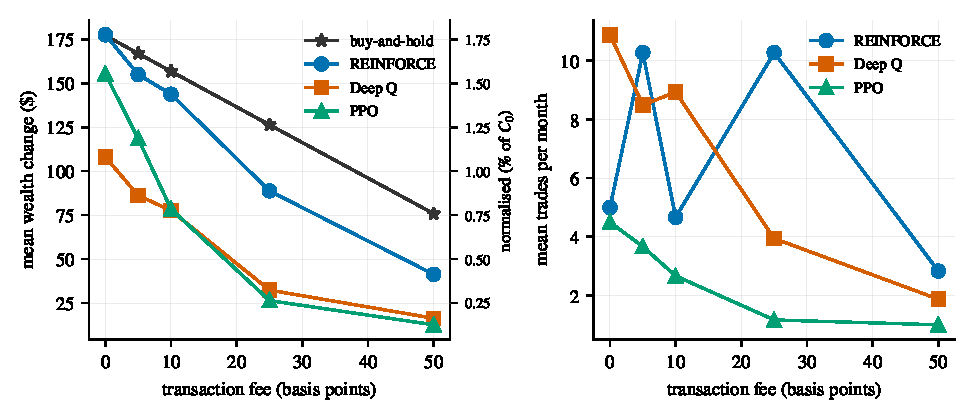
\includegraphics[width=0.95\textwidth]{figs5/fig5_fees.pdf}
  \caption{Fee sensitivity. Left: mean wealth change falls for every
  strategy as fees rise. Right: Deep Q-learning cuts its trading activity
  almost monotonically with the fee; PPO's trade count declines more
  gently; REINFORCE's trade counts move without pattern.}
  \label{fig:fees}
\end{figure}

\subsection{Effect of transaction costs on returns}

Raising the fee from 0 to 50 basis points cut buy-and-hold's return by
\$101.26 (from $+\$177.09$ to $+\$75.83$, a 57\% reduction), REINFORCE's
by \$136.25 (77\%), Deep Q-learning's by \$91.68 (85\%) and PPO's by
\$142.75 (92\%). Buy-and-hold's decline is itself an arithmetic check: its
\$101.26 loss is almost exactly the round-trip cost of its single
full-size position --- one \$10{,}000 buy and one matching sell at 0.5\%
each --- so the environment charges what it claims to charge. The learned
agents lose proportionally more because they trade more often, or, in
PPO's case, because higher fees push more of its seeds into near-inactivity
whose wealth change collapses with the cost.

\subsection{Effect of transaction costs on trading behaviour}

The behavioural content is in the trade columns. Deep Q-learning cut its
activity from 10.9 trades per month at zero fees to 1.9 at 50 basis points,
an 83\% reduction: as each action gets more expensive, the agent acts
less. PPO's mean trade count also falls, from 4.5 to 1.0, but the drop
(3.5 trades) sits inside its per-seed trade noise (5.0), so the decline is
directionally consistent rather than statistically decisive --- many PPO
seeds simply stop trading at high fees, which is why the mean return falls
sharply even though the mean trade count moves only gently. REINFORCE
shows no such adaptation --- its trade counts run 5.0, 10.3, 4.7, 10.3,
2.8 across the grid, and its per-seed variation in trade counts (up to
15.8 trades) swamps any trend. A policy that does not condition on the
state cannot adapt to a changed economic environment; the fee grid
re-detects the conditioning result of Section~5.4 by economic means.

\subsection{Robustness of the findings}

No qualitative conclusion of the chapter depends on the 5-basis-point
assumption. At every fee level, all three learned agents remain below
buy-and-hold, and the ordering between REINFORCE and Deep Q-learning is
unchanged. The fee experiment also supplies the chapter's clearest
evidence that a state-dependent agent responds to an economic property of
the environment, which matters for the discussion that follows.

\section{Discussion of the Main Findings}

This section synthesises the experiments against the five research
questions of Section~5.1.

\subsection{Learned agents did not outperform buy-and-hold}

On the held-out months the best learned return was $+\$171.51$ per month
against the benchmark's $+\$180.25$, and every other learned configuration
fell further behind. The result should be read against the structure of
the task: the test years rose, so full participation was already
near-optimal, and any agent that steps out of the market must recover the
return it sacrifices while in cash. The experiments found no agent that
could identify such moments reliably --- including in March 2025, the one
test month where stepping aside was most valuable. The implementations
themselves are not the cause: they learn on standard benchmarks and, as
Section~5.8 shows, at least one responds sensibly to costs.

\subsection{Adding drawdown information did not provide a clear advantage}

The nine-to-ten-feature comparison moved returns by $-\$4.12$ and
$+\$3.13$ for the two stable methods, both well inside seed spread, and
left the behavioural diagnostics unchanged. This does not imply the
nine-feature state is universally sufficient. It means that, within this
environment and under the wealth-change objective, drawdown information
provided no measurable advantage --- information is only worth using when
the objective rewards using it, and a wealth-maximising agent in rising
markets has little reason to consult its loss history. The pairing that
makes the feature relevant, the risk-aware reward, reduced participation
instead (Section~5.7).

\subsection{Lower risk was largely associated with lower exposure}

Every drawdown reduction in the chapter came with a near-proportional
exposure and return reduction, and no learned configuration sits above the
proportional lines of Figure~\ref{fig:effic}. Deep Q-learning's flagship
numbers --- 41\% of the benchmark return at 34\% of its exposure and 40\%
of its drawdown --- describe an agent that holds less, not one that avoids
worse. The March 2025 example sharpens this: in the benchmark's worst
month the state-dependent agent held \emph{more} than its average exposure
and lost in proportion. Distinguishing scaled-down participation from
genuine downside management requires exactly the exposure-relative reading
used here, and by that reading none of the agents managed downside risk.

\subsection{Algorithm choice affected how the state was used}

The sharpest divide in the results is behavioural. REINFORCE was
state-dependent in 0 of 6 seeds in every configuration tested; PPO managed
at most 2 of 6; Deep Q-learning achieved 6 of 6 in every wealth-reward
configuration. The divide changes how the returns must be read: without
the diagnostic, REINFORCE's $+\$171.51$ would look like the best learned
strategy, when it is an unconditional buy schedule that two rising years
paid well. Reporting returns without behavioural evidence would have led
this dissertation to the wrong conclusion.

\subsection{Action size materially affected achievable performance}

Two of the largest effects in the chapter came from the action model, not
from learning. The uncalibrated $0.10\,C_0$ slice capped attainable
exposure at 76\% of the benchmark's before any learning began, and the
whole-share and $0.10\,C_0$ variants moved test returns by up to \$101.60
per month --- two to three times the largest state-representation effect.
A benchmark comparison is only fair once the action model permits
comparable exposure, which is why the calibration preceded everything else
and why the action model belongs to the problem definition.

\subsection{Transaction costs influenced learned trading behaviour}

Deep Q-learning traded 83\% less as fees rose from 0 to 50 basis points,
PPO's mean trade count fell more gently (4.5 to 1.0) while its return
collapsed with cost, and REINFORCE's activity showed no systematic
response. The incentives encoded in the environment therefore transmit
clearly to the state-dependent learner, and more weakly to PPO. This
strengthens the overall interpretation: the failures documented above
are failures of what the objective rewards, not of the machinery that
optimises it.

\subsection{Implications for the research objectives}

Against the dissertation's central aim --- determining whether
reinforcement learning can learn profitable trading strategies for the
selected asset net of costs --- the experiments return a qualified
negative with a specific mechanism. Learning succeeded in the narrow
sense: implementations work, one agent uses the state, and behaviour
responds to costs. It failed in the economic sense: under a wealth-change
objective in rising markets, the optimal learned behaviours were either
unconditional participation (which needs no learning) or reduced
participation (which underperforms). The binding constraints identified
are the objective's incentives and the action model, not the state
representation --- a diagnosis that directly shapes the improvements
proposed in Chapter 6.

\section{Chapter Summary}

This chapter evaluated the trading agents against non-learning benchmarks
under a fixed protocol: decisions on validation months, one pass over 24
held-out months, six seeds per configuration. The action model was
calibrated first ($0.25\,C_0$, ceiling 0.838 against buy-and-hold's
0.910), because the original slice made the benchmark unreachable. The
conditioning diagnostic, run at both trade slices, then split the
algorithms categorically: the policy-gradient methods converged to
unconditional policies (1 of 24 REINFORCE and PPO seeds state-dependent),
while Deep Q-learning used the state in all 12 of its seeds.

On the held-out months no learned agent beat buy-and-hold's $+\$180.25$
per month. REINFORCE came closest ($+\$171.51$) by reproducing the slice
schedule; Deep Q-learning earned $+\$74.68$ at one-third of the
benchmark's exposure --- proportional scaling rather than timing, as its
lower Sharpe ratio confirms. Adding the drawdown feature moved returns by
less than \$5 per month for the stable methods. The risk-aware reward at
$\lambda = 0.10$ cut Deep Q-learning's drawdown by 41\% but its return by
32\% and its exposure by half, and the fee sweep showed the same agent
cutting its trading by 83\% as costs rose --- responsive behaviour, but
not profitable behaviour. Chapter 6 discusses the implications and
limitations of this design and the objectives that could reward
information use directly.
